\thesischapter{Background: The European Rail Traffic Management System}
\label{chapter:ERTMS}

Following the successful use of the solid state interlocking for over 30 years Railway Engineers are trying to employ modern technologies such as GPS and mobile data communications in the form of GSM radio to gain a much finer control than the traditional discrete solid state interlocking than their boolean track circuits alone would allow. This has led to the development of the European Rail Traffic Management System (ERTMS) which combines the traditional discrete control systems of the railway with continuous systems. The name ERTMS is often used interchangeably with the name \emph{European Train Control System} (ETCS) which is used to describe the same control system but without the GSM radio component. This new system consists of a \emph{radio block processor} (RBC) which negotiates with the traditional interlocking in order to grant lenghts of track to a train in the form of a \emph{movement authority} (MA). In this system every train has a movement authority which allocates it a length of track within which it can move. The RBC also provides the train with a \emph{static speed profile} which restricts the speed of the train on different segments of track. The trains are free to move along the lengths of track granted to them in the form of a MA and communicate their position, speed and requests for further segments of track over radio to the radio block processor. The ERTMS system is split into different levels of behaviour (See \ref{sec:theertms}.) that allow for different stages of delivery. In the most advanced level 3 all trains must be equipped with the ERTMS system in order to use the tracks, earlier levels allow for a mixture of trains with and without ERTMS. The RBC communicates with trains via GSM in ERTMS level 2 and 3 and via trackside balises in level 1. The interlocking itself is not formally considered to be a part of ERTMS, however an interface to the interlocking is a key part of this system. In this thesis we are mainly concerned with the ERTMS level 2 which in a later chapter is verified as part of a combined interlocking and RBC system.


\section{The European Rail Traffic Management System}
\label{sec:theertms}
\subsection*{ERTMS levels}
ERTMS is seperated into different levels of implementation. These range from being a compliment to traditional signalling to a complete replacement for it. Currently both, level 1 and 2, have been implemented in different parts of the world and level 3 is still in the conceptual phase and has yet to be implemented anywhere.

\textbf{ERTMS Level 1:} (Figure \ref{fig:ERTMSLevel1}) Movement authorites are calculated based on the underlying signalling system and then transmitted from the trackside to the train through the use of an electronic beacon called an Eurobalise.  The Eurobalise also enables train detection at the trackside and passes relevant information regarding train movement via the landside equipment unit (LEU) to the interlocking and signalling centre. While this level makes use of an interlocking,  it does not make use of a radio block controller unlike later levels of ERTMS.  \\



\begin{center}
\begin{figure}[h!]




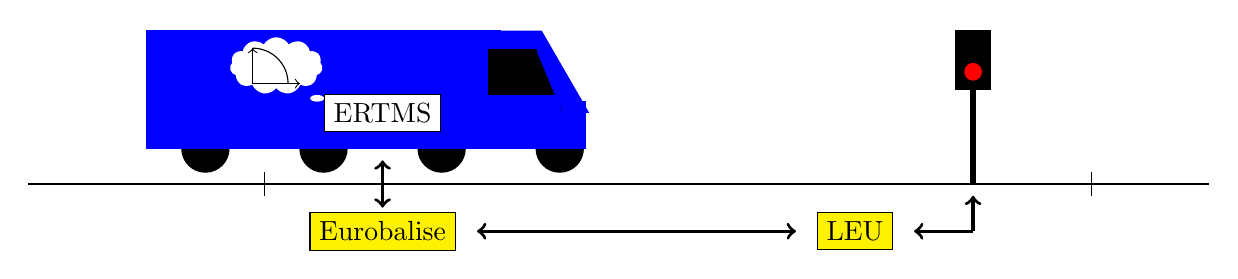
\begin{tikzpicture}[scale = 1.5]
\usetikzlibrary[shapes.geometric]
\usetikzlibrary[shapes.callouts]

%% Draw Wheels

\foreach  \a in {1  ,..., 4}{
	\filldraw [black]  (\a+0.5, 0) circle  (0.2cm);
}

%% Draw Carridge

\filldraw [blue] ( 1,0) rectangle (4, 1);

%% Draw Cab

\node[trapezium, fill = blue, minimum width = 2.25cm] at (4, 0.65) {};

\filldraw [blue] (4, 0.4) rectangle (4.72, 0);


\node[rectangle, black, fill = white, draw ] at (3, 0.3) {ERTMS};


%% Draw Windows
%
%\filldraw [black] (-1.5, 0.35) rectangle (-1.2, 0.8);
%
%\filldraw [black] (-0.7, 0.35) rectangle ( -0.4 , 0.8);
%
%\filldraw [black] (0.1 , 0.35) rectangle ( 0.4 , 0.8);
%
%

%%% Draw Cab Window

\filldraw [black] (3.9, 0.33 ) rectangle (4.3, 0.835);



\node[isosceles triangle, fill = black , minimum width = 0.63cm, shape border rotate = 90] at (4.3,0.45) {};

\filldraw [blue] (3.9,0.33) rectangle (4.5, 0.45);
%%% Draw ERTMS

\node[rectangle, black, fill = white, draw ] at (3, 0.3) {ERTMS};

\node[cloud callout, fill = white, cloud puffs  = 11, aspect = 2, cloud puff arc = 120, inner xsep = 0.4cm , callout relative pointer = {(0.315cm, -0.25cm)} ] at (2.1, 0.7) {};

\draw[->](1.9,0.55) -- (1.9,0.85);

\draw[->](1.9, 0.55) -- (2.3, 0.55 ) ;
\draw (2.2, 0.55) arc (0:90:0.3cm);


%%% Draw Track

\draw ( 0 , -0.3) -- (10 , -0.3);


\draw (2 , -0.4) -- (2 , -0.2);

\draw (9 , - 0.4) -- (9 , -0.2);

%%% Signal

\draw [line width = 2pt ] (8, -0.3) -- (8, 1);
\filldraw [black] (7.85, 1) rectangle (8.15, 0.5);

\filldraw [red] (8, 0.65) circle (2pt);
\filldraw [black] (8, 0.85) circle (2pt);


%%% Eurobalise
%
\node[rectangle, fill = yellow, minimum width = 1cm , draw] at (3, - 0.7) {Eurobalise};

\draw[<->, very thick] (3, -0.5 ) -- (3, -0.1 );

\node[rectangle, fill = yellow, draw] at (7, - 0.7) {LEU};

\draw[<->, very thick]  (3.8 , -0.7) -- (6.5,-0.7);

\draw[->, very thick ] (8, -0.7)  -- (8 , -0.4);

\draw[->, very thick] (8, - 0.7) -- (7.5 , -0.7);

\end{tikzpicture}



 \caption{ERTMS Level 1}
\label{fig:ERTMSLevel1}
\end{figure}
\end{center}

\textbf{ERTMS Level 2:}  (Figure \ref{fig:ERTMSLevel2}) This level of ERTMS is an intermediate stage in its deployment as it still contains some of the traditional discrete railway control systems. All implementations of ERTMS level 2 still make use of track circuits for the detection of trains. The traditional coloured light track side signals are optional in this level of implementation. They allow for non ERTMS trains to still run on the  track but coloured light signals can be removed if no such trains are running. Movement authorities are calculated based on the blocks contained in the underlying signalling system by the radio block processor which is located in the radio block centre. Data is continuously transmitted via radio between the radio block centre and the train in both directions. Movement authorities are transmitted to the train, which in return provides its location relative to a given balise. This transmission is complemented by on-the-spot transmission between the track side balise and the train. These track side balise act as both a beacon and a point of reference enabling the train to determine its location along the track. Train detection is also performed at the trackside using track circuits and axle counters, however these determine whether a segment of track is occupied for the purpose of route setting, rather than the exact location of the train. \



\begin{center}
\begin{figure}[h!]




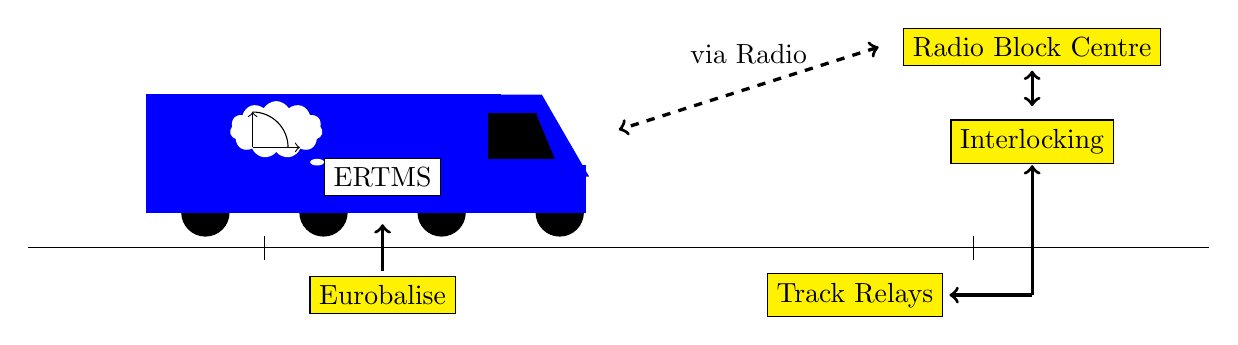
\begin{tikzpicture}[scale = 1.5]
\usetikzlibrary[shapes.geometric]
\usetikzlibrary[shapes.callouts]

%% Draw Wheels

\foreach  \a in {1  ,..., 4}{
	\filldraw [black]  (\a+0.5, 0) circle  (0.2cm);
}

%% Draw Carridge

\filldraw [blue] ( 1,0) rectangle (4, 1);

%% Draw Cab

\node[trapezium, fill = blue, minimum width = 2.25cm] at (4, 0.65) {};

\filldraw [blue] (4, 0.4) rectangle (4.72, 0);


\node[rectangle, black, fill = white, draw ] at (3, 0.3) {ERTMS};


%% Draw Windows
%
%\filldraw [black] (-1.5, 0.35) rectangle (-1.2, 0.8);
%
%\filldraw [black] (-0.7, 0.35) rectangle ( -0.4 , 0.8);
%
%\filldraw [black] (0.1 , 0.35) rectangle ( 0.4 , 0.8);
%
%

%%% Draw Cab Window

\filldraw [black] (3.9, 0.33 ) rectangle (4.3, 0.835);



\node[isosceles triangle, fill = black , minimum width = 0.63cm, shape border rotate = 90] at (4.3,0.45) {};

\filldraw [blue] (3.9,0.33) rectangle (4.5, 0.45);
%%% Draw ERTMS

\node[rectangle, black, fill = white, draw ] at (3, 0.3) {ERTMS};

\node[cloud callout, fill = white, cloud puffs  = 11, aspect = 2, cloud puff arc = 120, inner xsep = 0.4cm , callout relative pointer = {(0.315cm, -0.25cm)} ] at (2.1, 0.7) {};

\draw[->](1.9,0.55) -- (1.9,0.85);

\draw[->](1.9, 0.55) -- (2.3, 0.55 ) ;
\draw (2.2, 0.55) arc (0:90:0.3cm);


%%% Draw Track

\draw ( 0 , -0.3) -- (10 , -0.3);


\draw (2 , -0.4) -- (2 , -0.2);

\draw (8 , - 0.4) -- (8 , -0.2);


%%% Signal


%%% Eurobalise
%
\node[rectangle, fill = yellow, minimum width = 1cm , draw] at (3, - 0.7) {Eurobalise};

\draw[->, very thick] (3, -0.5 ) -- (3, -0.1 );

\node[rectangle, fill = yellow, draw] at (7, - 0.7) {Track \hfill
									      Relays};
%
%\draw[<->, very thick]  (3.8 , -0.7) -- (6.1,-0.7);

\draw[->, very thick ] (8.5, -0.7)  -- (8.5 , 0.4);

\draw[->, very thick] (8.5, - 0.7) -- (7.8 , -0.7);

\node[rectangle, fill = yellow, minimum width = 1cm , draw] at (8.5, 0.6) {Interlocking};

\draw[<->, very thick] (8.5 , 0.9) -- (8.5, 1.2);

\node [rectangle, fill = yellow, minimum width = 1cm, draw] at (8.5, 1.4){Radio \hfill Block \hfill Centre};

\draw[<->, very thick, dashed] (7.2 , 1.4) -- (5, 0.7) node [above = 5pt,midway] {via Radio};




\end{tikzpicture}



 \caption{ERTMS Level 2}
\label{fig:ERTMSLevel2}
\end{figure}
\end{center}


\textbf{ERTMS Level 3:}  (Figure \ref{fig:ERTMSLevel3})  Instead of using the block system based on track circuits from previous levels, the train itself is considered a moving block.  Route locking and route releasing are performed by the radio block centre using information gathered from trains. Similarily to ERTMS Level 2 communication takes place via radio between the train and the radio block centre. Integrity checking is performed on board of the train as it continuously monitors its position along the track.




\begin{center}
\begin{figure}[h!]




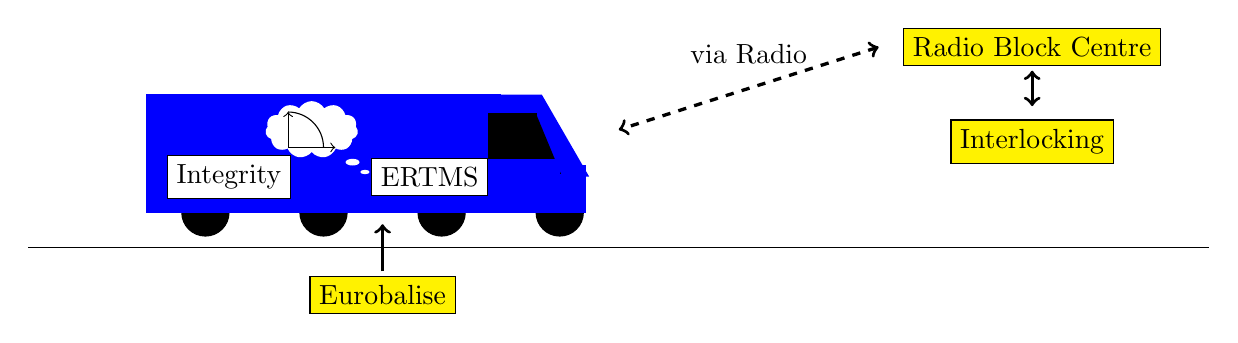
\begin{tikzpicture}[scale = 1.5]
\usetikzlibrary[shapes.geometric]
\usetikzlibrary[shapes.callouts]

%% Draw Wheels

\foreach  \a in {1  ,..., 4}{
	\filldraw [black]  (\a+0.5, 0) circle  (0.2cm);
}

%% Draw Carridge

\filldraw [blue] ( 1,0) rectangle (4, 1);

%% Draw Cab

\node[trapezium, fill = blue, minimum width = 2.25cm] at (4, 0.65) {};

\filldraw [blue] (4, 0.4) rectangle (4.72, 0);





%% Draw Windows
%
%\filldraw [black] (-1.5, 0.35) rectangle (-1.2, 0.8);
%
%\filldraw [black] (-0.7, 0.35) rectangle ( -0.4 , 0.8);
%
%\filldraw [black] (0.1 , 0.35) rectangle ( 0.4 , 0.8);
%
%

%%% Draw Cab Window

\filldraw [black] (3.9, 0.33 ) rectangle (4.3, 0.835);



\node[isosceles triangle, fill = black , minimum width = 0.63cm, shape border rotate = 90] at (4.3,0.45) {};

\filldraw [blue] (3.9,0.33) rectangle (4.5, 0.45);
%%% Draw ERTMS
\node[rectangle, black, fill = white, draw ] at (3.4 , 0.3) {ERTMS};

\node[cloud callout, fill = white, cloud puffs  = 11, aspect = 2, cloud puff arc = 120, inner xsep = 0.4cm , callout relative pointer = {(0.315cm, -0.25cm)} ] at (2.4, 0.7) {};

\draw[->](2.2,0.55) -- (2.2,0.85);

\draw[->](2.2, 0.55) -- (2.6, 0.55 ) ;
\draw (2.5, 0.55) arc (0:90:0.3cm);
\node[rectangle,fill = white, draw] at (1.7 , 0.3) {Integrity};

%%% Draw Track

\draw ( 0 , -0.3) -- (10 , -0.3);




%%% Signal


%%% Eurobalise
%
\node[rectangle, fill = yellow, minimum width = 1cm , draw] at (3, - 0.7) {Eurobalise};

\draw[->, very thick] (3, -0.5 ) -- (3, -0.1 );
%
%\node[rectangle, fill = yellow, draw] at (7, - 0.7) {Track \hfill
%									      Relays};
%
%\draw[<->, very thick]  (3.8 , -0.7) -- (6.1,-0.7);
%
%\draw[->, very thick ] (8.5, -0.7)  -- (8.5 , 1.2);
%
%\draw[->, very thick] (8.5, - 0.7) -- (7.8 , -0.7);
%
%\draw[->, very thick ] (8.5, -0.7)  -- (8.5 , 0.4);
%
%\draw[->, very thick] (8.5, - 0.7) -- (7.8 , -0.7);

\node[rectangle, fill = yellow, minimum width = 1cm , draw] at (8.5, 0.6) {Interlocking};

\node [rectangle, fill = yellow, minimum width = 1cm, draw] at (8.5, 1.4){Radio \hfill Block \hfill Centre};

\draw[<->, very thick, dashed] (7.2 , 1.4) -- (5, 0.7) node [above = 5pt,midway] {via Radio};


\draw[<->, very thick] (8.5 , 0.9) -- (8.5, 1.2);


\end{tikzpicture}



 \caption{ERTMS Level 3}
\label{fig:ERTMSLevel3}
\end{figure}
\end{center}


\subsection*{Static Speed Profile}
Traditionally the speed limit along a segment of track was controlled by a combination of speed limit signs at the side of the tracks. In ERTMS this has been replaced by a \emph{static speed profile} which provides the control system on the train with a maximum speed for a given section of track. Each type of train has its own static speed profile depending what it is capable of, for instance a high speed intercity train will have a different static speed profile from a fully loaded freight train. Proving the trains with a static speed profile increases safety further by making speeding less likely and allows for a finer control of the train's speed increasing the capacity of the line.

\subsection*{Movement Authority}
There are two different types of movement authorities used to restrict the movement of a train along a piece of track (See Figure \ref{fig:trackplan}).
\begin{description}

\item[End of Authority (EoA)] is the end of the movement authority for a train on a given piece of track. It is a point which the train can not proceed past along that track.

\item[Limit of Authority (LoA)]
 is a train's maximum allowed velocity (VMax) at a position on a piece of track and is calculated using breaking curves.

\end{description}

The on-board control system will automatically apply the brakes if the train exceeds either type of movement authority.



\begin{center}
\begin{figure}[h!]

\begin{sideways}
\begin{minipage}{25cm}

\begin{tikzpicture}

%%% Y Axis

\draw [->]
(-5 , 4) -- (-5,7)
node [left,text width=3cm,text centered,midway]
{ \hfill \\
VMax \\
(Limit of \\
Authority)
};

%%% X Axis

\draw [->]
(-5 , 4) -- (14,4)
node [below,text width=3cm,text centered,midway]
{ \hfill \\
Position
};


%%%% LoA Graph

\draw ( -2.80, 7) -- (-1, 7);


\draw(-1, 7) .. controls +(2 cm , - 0 cm) and +(-2 cm, 1.5 cm)
..  (8 , 4 );

%%% EoA

\draw [->]
(8 , 7) -- (8,5)
node [right,text width=3cm,text centered,midway]
{ \hfill \\
End of Authority
};




% Top Track


\draw (-5.10,2) -- (14, 2);

% Far Left Signal

\draw (-5,2) -- (-5, 2.25);
\draw (-5,2.25) -- (-4.75, 2.25);

\filldraw [red](-4.70, 2.25) circle (2pt) ;
\filldraw [black](-4.55, 2.25) circle (2pt) ;
\filldraw [black](-4.40, 2.25) circle (2pt);

% Mid Left  Signal

\draw (-1,2) -- (-1, 2.25);
\draw (-1,2.25) -- (-0.75, 2.25);

\filldraw [black](-0.70, 2.25) circle (2pt) ;
\filldraw [black](-0.55, 2.25) circle (2pt) ;
\filldraw [green](-0.40, 2.25) circle (2pt);

% Centre Signal


\draw (4,2) -- (4, 2.25);
\draw (4,2.25) -- (4.25, 2.25);

\filldraw [black](4.40, 2.25) circle (2pt) ;
\filldraw [yellow](4.55, 2.25) circle (2pt) ;
\filldraw [black](4.70, 2.25) circle (2pt);


% Mid Right Signal 

\draw (8,2) -- (8, 2.25);
\draw (8,2.25) -- (8.25, 2.25);

\filldraw [red](8.40, 2.25) circle (2pt) ;
\filldraw [black](8.55, 2.25) circle (2pt) ;
\filldraw [black](8.70, 2.25) circle (2pt);

% Far Right Signal 

\draw (12,2) -- (12, 2.25);
\draw (12,2.25) -- (12.25, 2.25);

\filldraw [black](12.40, 2.25) circle (2pt) ;
\filldraw [black](12.55, 2.25) circle (2pt) ;
\filldraw [green](12.70, 2.25) circle (2pt);



% Block Divisions

\draw (-4.10, 1.90) -- (-4.10 , 2.10);

\draw(-3.10, 1.90) -- (-3.10 , 2.10);

\draw(-2.10, 1.90) -- (-2.10, 2.10);




\draw(-1.30, 1.90) -- (-1.30, 2.10);



\draw(0.625, 1.90) -- (0.625, 2.10);




\draw(3, 1.90) -- (3, 2.10);


\draw(5, 1.90) -- (5, 2.10);

\draw(7, 1.90) -- (7, 2.10);

\draw(9, 1.90) -- (9, 2.10);

\draw(11, 1.90) -- (11, 2.10);

\draw(13, 1.90) -- (13, 2.10);



% Train 1

\draw [->]
(-2.80,1.4) -- (-2.80,1.8)
node [below,text width=3cm,text centered,midway]
{ \hfill \\
Train 1
};

% Train 2

\draw [->]
(10,1.4) -- (10,1.8)
node [below,text width=3cm,text centered,midway]
{ \hfill \\
Train 2
};

\end{tikzpicture}

\end{minipage}
\end{sideways}
\centering

 \caption{Movement Authorities in ERTMS Level 1}
\label{fig:trackplan}
\end{figure}
\end{center}


\subsection*{An Informal Description of the Combined System}
In the following we will present a high level description of the combined interlocking and radio block processor system.
The aim of specifying a combined system is to get rid of the inconsistencies and problems caused by the interface between the RBC and interlocking.  These are two seperate control systems each with its method of communicating instructions to the train. The interlocking acts a small safety kernel in the traditional train control system which should also be the case in the combined system, it must have the final say on any instruction to the trains or railtrack. If this is not the case then we may end up in a situation where a train is in a safe position according to one system but not the other. A prime example of such an inconsistency occurs when a high speed ERTMS enabled train travels along a line, under the guidance of a movment authority and is allowed to travel through an ordinary red light.  

 The components of the system which we are trying to capture can be found inside the dotted line in figure \ref{fig:ERTMSCombine}. These consist of the interlocking and radio block processor. Currently the interface between them is biased in one direction, most of the information travels from the interlocking to the radio block processor. Some information does go in the other direction; for example the radio block centre will notify the interlocking when a ERTMS enabled train is travelling along the line.  However, other possibilities for a partition in a combined system exist, for example the route setting and releasing could take place in the radio block centre. There are also different possibilities from the level of partitioning/ integration of the system, it could be the case that a fully integrated system is much simplier, however such a system would have to be constructed from scratch. 



\begin{center}
\begin{figure}[h!]




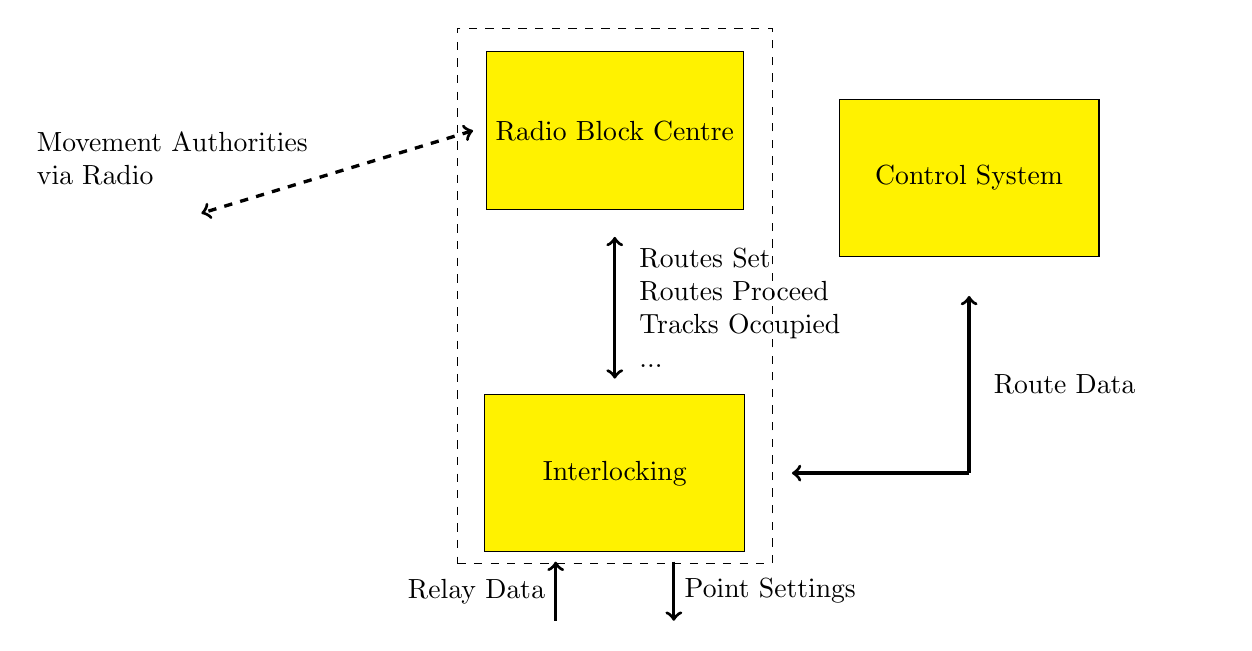
\begin{tikzpicture}[scale = 1.5]
\usetikzlibrary[shapes.geometric]
\usetikzlibrary[shapes.callouts]




%%% Signal


%%% Eurobalise
%%
%\node[rectangle, fill = yellow, minimum width = 1cm , draw] at (3, - 0.7) {Eurobalise};
%
%\draw[<->, very thick] (3, -0.5 ) -- (3, -0.1 );
%
%\node[rectangle, fill = yellow, draw] at (7, - 0.7) {Track \hfill
%									      Relays};
%
%\draw[<->, very thick]  (3.8 , -0.7) -- (6.1,-0.7);
%
%
%
%
\draw[<->, very thick ] (8.5, -0.7)  -- (8.5 , 0.5) node [right = 5pt, text width = 2.8 cm, midway] {Routes Set Routes Proceed Tracks Occupied ...};

%%\draw[->, very thick] (8.5, - 0.7) -- (7.8 , -0.7);



\node [rectangle, fill = yellow, minimum width = 1cm, minimum height = 2cm, draw] at (8.5, 1.4){Radio \hfill Block \hfill Centre};





\node [rectangle, fill = yellow, minimum width = 3.3cm, minimum height = 2cm, draw] at (8.5, -1.5){Interlocking};




\draw[<->, very thick, dashed] (7.3 , 1.4) -- (5, 0.7) node [above = 5pt, left = 5pt, text width = 3.5 cm, midway] {Movement Authorities via Radio};

\draw[<- , very thick] (10, -1.5)  -- (11.5, - 1.5);

\draw[-> , very thick] (11.5, -1.5) -- ( 11.5, 0) node [right = 5pt, text width = 2.8 cm, midway] {Route Data};


\draw[<- , very thick]  (8, - 2.25) -- (8, -2.75) node [left, midway] {Relay Data};


\draw[-> , very thick]  (9, - 2.25) -- (9, -2.75) node [right, midway] {Point Settings};

\node[rectangle, minimum width = 4cm, minimum height = 6.8cm, dashed, draw] at (8.5, 0) {};

\node [rectangle, fill = yellow, minimum width = 3.3cm, minimum height = 2cm, draw] at (11.5, 1){Control System};

\end{tikzpicture}



 \caption{Current Situation}
\label{fig:ERTMSCombine}
\end{figure}
\end{center}

We will make the following assumptions in the modelling of the combined system:

\begin{itemize}

\item We assume that positioning works and that the location of the trains is known at all times.

\item We assume that all trains are fitted with the ERTMS system.

\item We will only work with one radio block controller. Trains are assumed to enter and exit the controlled area.


\end{itemize}

As part of this project we will also have to formalise new safety properties for the combined system. Some of examples of these are as follows:

\begin{itemize}

\item A point should not move if it is in a movement authority

\item Two trains should not have over lapping movement authorities

\end{itemize}


\section{Typical  ERTMS Scenario}

Consider the following scenario involving 3 trains attempting to cross a double junction (See Fig \ref{fig:trackplan}).

\begin{itemize}
\item Train A would like to travel in a route from D to C
\item Train B would like to travel in a route from A to B
\item Train C would like to travel in a route from F to C
\end{itemize}

We will assume that initially no routes are set. This means that either a controller or a time table will determine the precedence of the trains. For this example we will time table the trains in alphabetical order.



\begin{figure}[H]

\begin{center}

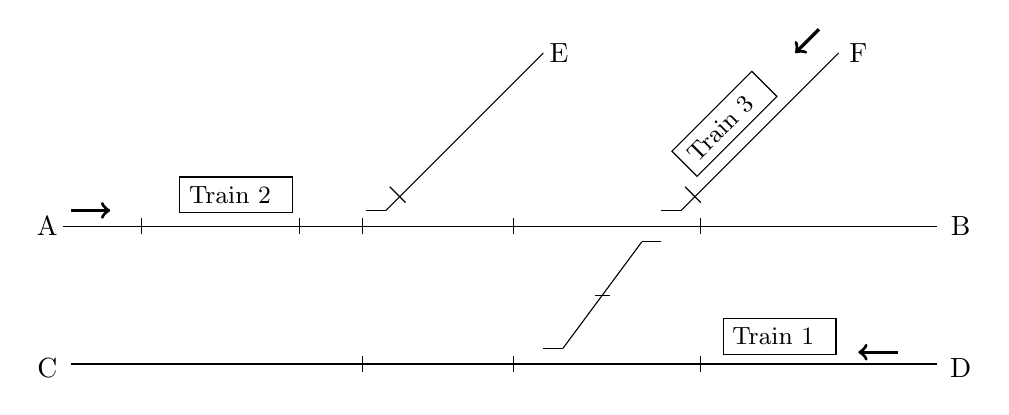
\begin{tikzpicture}

% Top Track

\draw (-5.10,2) -- (6,2);

% Segment Divide 8023/8201

\draw (-4.10, 1.90) -- (-4.10 , 2.10);



%%% Trains

\tikzstyle{train}=[rectangle, draw, text width = 1.2cm, font=\small]


\node (A) [train]  at (4, 0.6)                  {Train 1
                                            };

\node(B)[train] at (-2.9, 2.4) {Train 2}; 

\node(C)[train,rotate = 45] at (3.3,3.3) {Train 3};


%%% Route Markers

\node (D) at (-5.3, 2) {A};
\node (E) at (6.3, 2) {B};
\node (F) at (-5.3, 0.2) {C};
\node (G) at (6.3, 0.2) {D};
\node (H) at (5 ,4.20) {F};
\node (I) at (1.20,4.20) {E};

% Segment Divide 

\draw(-2.10, 1.90) -- (-2.10, 2.10);

%\draw(-2.10, 0.15) -- (-2.10 , 0.35);



% Segment Divide

\draw(-1.30, 1.90) -- (-1.30, 2.10);

\draw(-1.30, 0.15) -- (-1.30, 0.35);


% Left set of points

\draw (-1.25, 2.20) -- (-1, 2.20);

\draw (-1, 2.20) -- (1 ,4.20);

\draw (-0.75, 2.30) -- (-0.95, 2.50 ); 


% Segment Divide

\draw(0.625, 1.90) -- (0.625, 2.10);
\draw(0.625, 0.15) -- (0.625, 0.35);

%Right set of points%


\draw (2.5, 1.80) -- (2.25, 1.80);

\draw (2.25, 1.80) -- (1.25 ,0.45);

\draw (1.25,0.45) -- (1,0.45);

\draw (1.65 ,1.125) -- (1.85, 1.125);



% Left set of points

\draw (2.5, 2.20) -- (2.75, 2.20);

\draw (2.75, 2.20) -- (4.75 ,4.20);

\draw (3, 2.30) -- (2.80, 2.50 ); 
% Segment Divide

\draw(3, 1.90) -- (3, 2.10);

\draw(3, 0.15) -- (3, 0.35);



% Bottom Track
\draw (-5,0.25) -- (6, 0.25);



% Track Directions


\draw [->, very thick]
(-5,2.2) -- (-4.5,2.2);


\draw [->, very thick]
(5.5,0.4) -- (5,0.4);


\draw [->, very thick]
(4.5,4.5) -- (4.2,4.2);



\end{tikzpicture}

\end{center}

 \caption{A Common Scenario}
\label{fig:trackplan}
\end{figure}




\begin{figure} [H]

\begin{center}
\begin{tikzpicture}[node distance = 3cm, scale = 1.5]
\tikzstyle{arrow}=[->,shorten >=7pt,shorten <=7pt]



\draw (0,10) --  (0,0);

\draw (2, 10) -- (2, 0);

\draw (4, 10) -- (4, 0);

\draw (6, 10) -- (6, 0);

\draw (8,10 ) -- (8, 0);

\node[] at (0, 10.5) {RBC};
\node[] at (2, 10.5) {Interlocking};
\node[] at (4, 10.5) {Trackside};
\node[] at (6, 10.5) {Train 1};
\node[] at (8, 10.5) {Train 2};

\draw[->](0, 9.5) -- node[above, font = \small ]{Route Req} (2, 9.5);
\draw[<-](0, 9) -- node[above, font = \small]{Route Ack}(2,9); 
\draw[-](0,8.5) -- node[above, font = \small]{Points Set} (2, 8.5);
\draw[->](0,8.5) -- node[above, font = \small]{} (4, 8.5);
\draw[-](2, 8) -- node[above , font = \small]{Points Ack} (4, 8);  
\draw[<-](0, 8) -- node[above , font = \small]{} (4, 8);  

\draw[->](0,7.5) -- node[above, font = \small]{MA D $\to$ C} (6, 7.5);
\draw[<-](0, 7) -- node[above, font = \small]{MA Ack} (6, 7);  
\draw[<-](0, 6.5) -- node[above, font = \small]{Position Rep} (6, 6.5);  


\draw[->](0, 5) -- node[above, font = \small ]{Route Req} (2, 5);
\draw[<-](0, 4.5) -- node[above, font = \small]{Route Ack}(2,4.5); 
\draw[-](0,4) -- node[above, font = \small]{Points Set} (2, 4);
\draw[-](2, 3.5) -- node[above, font = \small]{Points Ack} (4, 3.5); 
\draw[->](0,4) -- node[above, font = \small]{} (4, 4);
\draw[<-](0, 3.5) -- node[above, font = \small]{} (4, 3.5);  
\draw[-](0,3) -- node[above, font = \small]{MA A $\to$ B} (2, 3);
\draw[->](0,3) -- node[above, font = \small]{} (8, 3);




%\draw [arrow] (0,9) -- node[above = 7pt] {Comm Sess Init} (7 ,7 );
%
%\draw [arrow] (7,6.5) -- node[above = 7pt] {System Version} (0 , 4.5);
%\draw [arrow] (0,4) -- node[above = 8pt, text width = 3.3cm] {Report and Tele No (Compatable)}  (7 ,2 );
%\node[text width = 3.5cm] at (3.5, 2) {Version Incompatable (Incompatable)};
%
%\node[rectangle,draw] at (-2 , 4.25) {Check Compatibility};
%\draw [arrow] (-0.5,4) -- node [left, text width = 2 cm] {Connection Established (Compatable)}  (-0.5, 0);
% \draw [arrow] (7.5,2) -- node [right, text width = 2 cm] {Connection Established (Compatable)}  (7.5, 0);


\end{tikzpicture}
\end{center}

\caption{Message Sequence Chart for "A Common Scenario"}
\label{fig:ContactOrders}
\end{figure}

\section{Previous Work: Attempts to Verify ERTMS}

